\documentclass[a4paper]{report}

\usepackage{natbib}
\bibpunct{[}{]}{,}{a}{}{;}
\usepackage{fancyheadings}
\usepackage{iamdip}
\usepackage[pdftex]{graphicx}
\usepackage{caption}
\usepackage{subcaption}
\usepackage{amsmath}
\usepackage{amsthm}
\usepackage{amssymb}
\usepackage{amsfonts}
\usepackage{url}
\usepackage{hyperref}
\usepackage{array}

\usepackage{pdfpages}

\usepackage{listings}
\usepackage{xcolor}

\usepackage{pdflscape}
\usepackage{afterpage}

\definecolor{dkgreen}{rgb}{0,0.6,0}
\definecolor{gray}{rgb}{0.5,0.5,0.5}
\definecolor{mauve}{rgb}{0.58,0,0.82}

\lstdefinestyle{inline}
{
numbers=left,
xleftmargin=1cm,
belowskip=3mm,
moredelim=**[is][\color{red}]{\$}{\$},
moredelim=**[is][\color{green}]{^}{^}
}

\lstdefinestyle{table}
{
numbers=none,
xleftmargin=0mm,
belowskip=0mm,
moredelim=**[is][\color{red}]{\$}{\$},
moredelim=**[is][\color{green}]{^}{^}
}

\lstset{frame=none,
  language=Java,
  aboveskip=3mm,
  showstringspaces=false,
  columns=flexible,
  basicstyle={\small\ttfamily},
  numberstyle=\tiny\color{gray},
  keywordstyle=\color{blue},
  commentstyle=\color{dkgreen},
  stringstyle=\color{mauve},
  breaklines=true,
  breakatwhitespace=true,
  tabsize=3,
  style=table
}


\headrulewidth 0.5pt \addtolength{\headheight}{5pt}

\lhead[\fancyplain{}{\rm\thepage}]{\fancyplain{}{\rightmark}}
\rhead[\fancyplain{}{\leftmark}]{\fancyplain{}{\rm\thepage}}
\cfoot{}

% \graphicspath{{../Figures/}}
\graphicspath{ {images/} }

\DeclareMathOperator{\score}{score}

\begin{document}

\pagestyle{fancyplain} \thispagestyle{empty}

\title{TITLE}
\author{Sven Kellenberger}
\betreuer{Prof. Dr. Paolo Favaro}
\ort{Bern}
\datum{01.08.2018}

\pagenumbering{roman} \setcounter{page}{1}
\maketitle

\newpage
\thispagestyle{empty}
\vspace{8cm}
\noindent
{\centerline {\bf \large Abstract}}
\vspace{1cm}


\noindent

\noindent This thesis covers the implementation of an LSTM based sequence-to-sequence model with an attention mechanism on top as well as the difficulties of introducing errors into source code that have the requirement to be as close to reality and as sophisticated as possible. The model is then trained to detect and correct these artificially introduced syntax, semantic and logic errors. This thesis also provides experimental evaluations of several architectural design choices and a detailed analysis of the introduced errors. The model achieves promising results for all generated errors and manages to gain some understanding of the semantics of source code. However, it could not be conclusively determined if the model is also able to learn to detect and correct logic errors. 


\pagenumbering{roman} \setcounter{page}{1}
\tableofcontents
\newpage{\pagestyle{empty} \cleardoublepage}

\pagenumbering{arabic} \setcounter{page}{1}
\pagestyle{fancy}

\chapter{Introduction}
\section{Motivation}
Automatic text correction is a ubiquitous technology in our today world. Every smartphone, every word processing software, every browser provides some form of error detection and correction for text input. These systems rely on a vocabulary of correct words or some machine learning algorithm to find errors and possible corrections.

Obviously similar techniques can also be applied to source code. The syntax of a programming language is strictly defined which enables integrated development environments (IDEs) to detect syntax errors before the program is even run. Of course the IDE's possibilities are limited by the properties of the programming language, e.g. is it strongly typed or weakly typed. However it is impossible to work with a fixed vocabulary because the naming of variables, methods, etc. is not restricted to a particular spelling (except for keywords).

Furthermore, the error detection in source code is mostly limited to syntax errors, while semantic errors show only at runtime if at all. These errors are also the hardest ones to fix. In a strongly typed language like Java, a lot of possible errors in naming and accessing attributes can be eliminated, because each variable has to be initiated before it is used and the type of the variables is known at all times and therefore also their available attributes and methods. In weakly typed languages like Ruby however, one can not determine what type of object a variable holds before runtime. This creates additional sources of runtime errors.

Insert neural networks. Deep neural networks have proved to be very effective in such tasks that are infeasible to solve with traditional algorithms.

The aim of this project is it to train a character based sequence-to-sequence model on the task of source code correction. The implementation of the model is based on the neural machine translation (NMT) model provided by Tensorflow \cite{seq2seq_tutorial}. As a dataset the Java Github Corpus \cite{java_dataset} is used as a source of correct data. This data is then perturbed as random syntax and semantic errors are added. The performance of different model architectures is then evaluated for the introduced errors.

\section{Outline}

\newpage{\pagestyle{empty} \cleardoublepage}

\chapter{Background}
\section{Software-based Approaches}

\section{Machine-learning-based Approaches}

\newpage{\pagestyle{empty} \cleardoublepage}

\chapter{Model and Training}
\section{Components}

This section aims to give a short overview of the main techniques and architectures used in this thesis. Different types of recurrent neural networks are discussed as well as the sequence-to-sequence model and the attention mechanism. All these architectures are essential parts of the model used in this thesis.

\subsection{Types of Recurrent Neural Networks}
\label{rnn_types}

\begin{figure}[p]
\centering
\includegraphics[width=0.9\linewidth]{rnn}
\caption{Architecture of a vanilla recurrent neural network cell. Each timestep some output and a hidden state vector \(\mathbf{h}_t\) are produced by looking at the hidden state vector from the previous timestep \(\mathbf{h}_{t-1}\) and the current input \(\mathbf{x}_t\). In this simple example, \(\mathbf{h}_t\) is also the output.}
\label{rnn}
\end{figure}

A recurrent neural network (RNN)\cite{rnn} is a special form of neural network that is used for sequential tasks. It works by having multiple copies of the network, one for each timestep. As the input proceeds in time, the network passes information to its next instance as seen in Figure \ref{rnn}. For an input sequence \((\mathbf{x}_1, ..., \mathbf{x}_n)\) a very simple RNN produces at each timestep \(t\) a hidden state vector \(\mathbf{h}_t\) as follows:

\begin{equation*}
  \mathbf{h}_t = \tanh \left(\mathbf{W} \begin{pmatrix} \mathbf{x}_t \\ \mathbf{h}_{t-1} \end{pmatrix} \right)
\end{equation*}

\begin{figure}[p]
\centering
\includegraphics[width=0.9\linewidth]{lstm}
\caption{Architecture of a typical LSTM cell. In addition to the hidden state vector \(\mathbf{h}_t\), a memory state vector \(\mathbf{c}_t\) is passed to the next timestep. \(\mathbf{h}_{t-1}\) and the input \(\mathbf{x}_t\) are used to compute the gates \(\mathbf{f}_t\), \(\mathbf{i}_t\) and \(\mathbf{o}_t\) and the candidate vector \(\mathbf{g}_t\). The gates are then used to add, delete and retrieve information to respectively from \(\mathbf{c}_{t-1}\), subsequently generating \(\mathbf{c}_t\) and \(\mathbf{h}_t\).}
\label{lstm}
\end{figure}

However, vanilla RNNs have proven to be hard to train and to struggle with long-range dependencies \cite{hochreiter_rnn}. In theory, they should be able to deal with these dependencies but either vanishing or exploding gradients usually prevent them from doing so. These issues were addressed with the introduction of Long Short-Term Memory networks (LSTMs) \cite{lstm}. In addition to \(\mathbf{h}_t\), LSTMs also pass a memory state vector \(\mathbf{c}_t\) to the next instance as can be seen in Figure \ref{lstm}. The LSTM can choose at each timestep which information it wants to read or forget from the memory vector or which new one it wants to write onto the vector. This is done by using explicit gating mechanisms:

\begin{align*}
  \mathbf{f}_t &= \sigma \left(\mathbf{W}_f \begin{pmatrix} \mathbf{x}_t \\ \mathbf{h}_{t-1} \end{pmatrix} \right) &
  \mathbf{i}_t &= \sigma \left(\mathbf{W}_i \begin{pmatrix} \mathbf{x}_t \\ \mathbf{h}_{t-1} \end{pmatrix} \right) \\
  \mathbf{o}_t &= \sigma \left(\mathbf{W}_o \begin{pmatrix} \mathbf{x}_t \\ \mathbf{h}_{t-1} \end{pmatrix} \right) &
  \mathbf{g}_t &= \tanh \left(\mathbf{W}_g \begin{pmatrix} \mathbf{x}_t \\ \mathbf{h}_{t-1} \end{pmatrix} \right)
\end{align*}

Here \(\sigma\) is the sigmoid function. \(\mathbf{f}_t\), \(\mathbf{i}_t\) and \(\mathbf{o}_t\) can be thought of as binary gates that decide which information from \(\mathbf{c}_{t-1}\) should be deleted, which information of \(\mathbf{c}_{t-1}\) should be updated and which information from \(\mathbf{c}_t\) should be written to \(\mathbf{h}_t\). Finally, \(\mathbf{g}_t\) is a vector of possible values that (gated by \(\mathbf{i}_t\)) can be added to \(\mathbf{c}_{t-1}\). The state vectors are then updated as follows:

\begin{align*}
  \mathbf{c}_t &= \mathbf{f}_t \odot \mathbf{c}_{t-1} + \mathbf{i}_t \odot \mathbf{g}_t \\
  \mathbf{h}_t &= \mathbf{o}_t \odot \tanh(\mathbf{c}_t)
\end{align*}

\begin{figure}[t]
\centering
\includegraphics[width=0.9\linewidth]{gru}
\caption{Architecture of a typical GRU cell. \(\mathbf{h}_{t-1}\) and the input \(\mathbf{x}_t\) are used to compute the reset gate \(\mathbf{r}_t\) and the update gate \(\mathbf{u}_t\). These gates are then used to compute a candidate vector \(\mathbf{h}_t'\) which in turn is then used to compute the new hidden state vector \(\mathbf{h}_t\).}
\label{gru}
\end{figure}

A more recent approach to optimizing RNNs are Gated Recurrent Units \cite{gru}. They have fewer parameters than LSTMs and work without an additional memory vector and are therefore faster to train and more light-weight (see Figure \ref{gru}). Recent research suggests that the performances of LSTM networks and of GRU networks are comparable \cite{lstm_vs_gru}.

In contrast to an LSTM, a GRU cell only has two gates, a reset gate \(\mathbf{r}_t\) and an update gate \(\mathbf{u}_t\). They are computed in a similar way as the gates of an LSTM:

\begin{align*}
  \mathbf{r}_t &= \sigma \left(\mathbf{W}_r \begin{pmatrix} \mathbf{x}_t \\ \mathbf{h}_{t-1} \end{pmatrix} \right) \\
  \mathbf{u}_t &= \sigma \left(\mathbf{W}_u \begin{pmatrix} \mathbf{x}_t \\ \mathbf{h}_{t-1} \end{pmatrix} \right)
\end{align*}

These gates are than used to calculate a candidate vector \(\mathbf{h}_t'\) of possible new values which is then used to compute the updated hidden state vector \(\mathbf{h}_t\).

\begin{align*}
  \mathbf{h}_t' &= \tanh \left(\mathbf{W}_{h'} \begin{pmatrix} \mathbf{x}_t \\ \mathbf{r}_t \odot \mathbf{h}_{t-1} \end{pmatrix} \right) \\
  \mathbf{h}_t &= (1 - \mathbf{u}_t) \odot \mathbf{h}_{t-1} + \mathbf{u}_t \odot \mathbf{h}_t'
\end{align*}

Almost all state of the art results today are achieved using either LSTMs, GRUs or similar networks with some form of gating mechanism because they are easier to train than vanilla RNNs and excel at capturing long-range dependencies.

\subsection{The Sequence-to-Sequence Model}

\begin{figure}[t]
\centering
\includegraphics[width=0.9\linewidth]{seq2seq}
\caption{The sequence-to-sequence model applied to a translation example. The English source sentence is fed to the model word by word. After the input of an end-of-sequence token (\texttt{<eos>}), the network starts producing the output sentence in French. For this, the produced output tokens are fed back to the network at the next timestep. The network signals the end of the sequence by outputting another \texttt{<eos>} token.}
\label{seq2seq}
\end{figure}

Traditional deep neural networks process the whole input in one step and then calculate some output, e.g. process an image and then classify it. This works well for problems where the input and the output are of a fixed dimension, however, it is not suitable for problems where the input and the output are sequences of variable length. An example would be the input of a question and the network should produce an answer. We have seen that we can use LSTMs to process input sequences of variable length. However, in this case we want to process the whole input sequence and all the information that comes with it first and only then start generating an output sequence. These problems are called sequence to sequence problems.

In \cite{seq2seq} the Sequence-to-Sequence Model is introduced as a solution to these problems. The model was applied to the task of neural machine translation (NMT) and has since become the state of the art architecture in this field. The main concept can be seen in Figure \ref{seq2seq}. First, the whole input sequence is fed into the network and the output is ignored. Then an end-of-sequence token \texttt{<eos>} is input which signals the network to start producing the output. From there on the produced output tokens are fed to the network until another an end-of-sequence token is generated, thus signaling the end of the sequence. To speed up training the expected output is fed back to the network and not the actually produced output.

This architecture is further improved by splitting the network into two separate LSTMs. The first network takes all the input and encodes it into its hidden state vector which is then used to initialize the second network which is first fed a start token \texttt{<GO>} and then the generated output until the end of the sequence is reached.

These networks usually operate at word level and use some word embedding like word2vec \cite{word2vec}. This method has the advantage of giving the input words some meaning through the embedding instead of just inputting a meaningless encoding of the word. While this is very effective for translation tasks, there are some limitations to this method. Embeddings work on a fixed size vocabulary which means that out of vocabulary words (OOV) can't be handled. Also special character sequences like \texttt{:)} pose a problem.

\subsection{Attention-Mechanism}

Attention is a relatively new concept for neural networks. The idea is to allow the network to chose on which information to focus at any given moment. For example in \cite{visual_attention} attention is used on the task of high resolution image classification. These kinds of networks often struggle with memory constraints and attention can help them to only load the significant part of the image into the memory.

Attention has subsequently been applied to NMT \cite{attention_bahdanau,attention_luong}. The vector into which the input is encoded in the sequence-to-sequence model has been identified as a bottleneck which cuts down performance because of its limited capacity. After all the vector is of fixed dimensionality and needs to encode information about the whole input sequence. Because of that attention is used as a way for the decoder to peek at previous hidden states of the encoder. This is done with a context vector \(\tilde{\mathbf{c}}_t\) which is combined with the current hidden state of the decoder \(\mathbf{h}_t\). The resulting attentional hidden state \(\tilde{\mathbf{h}}_t\) is then used by the decoder to generate the next output.

\begin{equation*}
  \tilde{\mathbf{h}}_t = \tanh \left(\mathbf{W}_c \begin{pmatrix} \tilde{\mathbf{c}}_t \\ \mathbf{h}_{t} \end{pmatrix} \right)
\end{equation*}

For the derivation of the context vector \(\tilde{\mathbf{c}}_t\) all hidden states \(\bar{\mathbf{h}}_s\) of the encoder are considered. For this, an alignment vector \(\mathbf{a}_t\) whose size equals the input sequence length is derived from the current decoder hidden state \(\mathbf{h}_t\) and the encoder hidden states \(\bar{\mathbf{h}}_s\). The values of \(\mathbf{a}_t\) are normalized using the softmax function.

\begin{equation*}
  a_{ts} = \frac
            {\exp(\score(\mathbf{h}_t, \bar{\mathbf{h}}_s))}
            {\sum_{s'} \exp(\score(\mathbf{h}_t, \bar{\mathbf{h}}_{s'}))}
\end{equation*}

Here, \(\score\) is a content-based function used to compare the decoder hidden state \(\mathbf{h}_t\) with each one of the encoder hidden states \(\bar{\mathbf{h}}_s\). There are various possible choices for this function, for example:

\begin{equation*}
  \score(\mathbf{h}_t, \bar{\mathbf{h}}_s) =
  \begin{cases}
    \mathbf{h}_t^\intercal \mathbf{W}_a \bar{\mathbf{h}}_s \\
    \mathbf{v}_a^\intercal \tanh \left(\mathbf{W}_a \begin{pmatrix} \mathbf{h}_t \\ \bar{\mathbf{h}}_s \end{pmatrix} \right)
  \end{cases}
\end{equation*}

The context vector \(\tilde{\mathbf{c}}_t\) is then calculated as the weighted average over the encoder hidden states.

\begin{equation*}
  \tilde{\mathbf{c}}_t = \sum_{s'} a_{ts'} \bar{\mathbf{h}}_{s'}
\end{equation*}

\section{Model Implementation}

The implementation of the model used in this thesis is mostly based on the NMT model from Tensorflow \cite{seq2seq_tutorial}. The model consists of an encoder and a decoder with an implementation of the Luong attention mechanism \cite{attention_luong} on top. The encoder and the decoder are both an LSTM cell consisting of 4 layers \`a 256 units each. No embedding was used because the model operates at the character level instead of the word level and a single character doesn't have much meaning without its context. This change was necessary because programming languages don't have a fixed vocabulary. The programmer is not restricted in the naming of variables, methods or the like and thus it makes no sense to restrict the model to a fixed vocabulary. Otherwise, it would only result in a lot of OOV tokens. Therefore the input is fed one character at a time to the model with the encoding of the character simply being its ASCII code, i.e. a number between 0 and 127.

For inference, the decoder was first fed a start-of-sequence token and after that the produced output was fed back as an input to the decoder until an end-of-sequence token was output. During training, however, the correct target sequence was fed to the decoder, left padded by a start-of-sequence token to optimize training.

 During backpropagation, the gradients were clipped by a fixed norm. This technique is used to prevent the gradients from exploding \cite{gradient_clipping}. The norm chosen for this thesis is 5 but other values would also be possible (1 would be another common choice).

 The loss was measured with the cross-entropy loss function. Each timestep the decoder produces some output vector \(\mathbf{y}'^\intercal = \begin{pmatrix} y_1' & ... & y_n'\end{pmatrix}\). This vector is then normalized using the softmax function to get probabilities \(p_i\) for each possible output.

 \begin{equation*}
   p_i = \frac
             {\exp(y_i')}
             {\sum_{j} \exp(y_j')}
 \end{equation*}

 These probabilities are then used to compute the cross-entropy loss:

 \begin{equation*}
   l = - \sum_{j} y_j * \log(p_j)
 \end{equation*}

 Here \(\mathbf{y}^\intercal = \begin{pmatrix} y_1 & ... & y_n \end{pmatrix}\) is a one-hot target vector with \(y_i = 1\) for the desired output \(i\) and \(y_j = 0\) everywhere else.

 For each setting, training was done for 30,000 iterations while the batch size was set to 64. The max sequence length was set to 300 meaning that only examples of 300 characters or less were used to train and evaluate the model.

\section{Dataset Construction}

To train the model, a big dataset of erroneous code examples produced by real programmers including their respective corrections would be ideal. This would assure a large variety of errors and real-life examples. However, such a dataset does not exist in part because the correction of erroneous code is a long and tedious work which has to be done by hand.

The best alternative is to take a dataset of correct code and introduce the errors artificially. This task is no trivial one and several difficulties have to be taken into account and weighed up against each other. For one, the more sophisticated an error is the harder it is to introduce it consistently, but training a network on only easy errors (like missing semicolons) doesn't produce any added value. Another issue is the artificiality of the errors. One runs the risk of the model picking up on the error generation patterns and thus performing poorly on non-artificial examples. These problems are further discussed in Subsection \ref{corruption}.

For this thesis, the data from the Java Github Corpus \cite{java_dataset} was chosen. As elaborated in Section \ref{code_correction_section}, a weakly typed programming language like Python would be preferable over a strongly typed one like Java because a lot of errors in Java can already be found algorithmically. However, there is a general lack of large, diverse datasets of source code thus the selection of the Java Github Corpus. Furthermore, this thesis doesn't aim at building a fully polished "code corrector" but rather tries to test the boundaries of the possible. The model knows nothing of the structure and rules of the programming language and therefore the capability of the model to grasp certain concepts can still be tested.

The dataset was crawled from Github and includes only projects which were forked at least once to assure a certain measure of quality. It consists of around 15,000 projects which amount to approximately 15GB of data.

\subsection{Preprocessing}

Before the data was used, some preprocessing had to be done. While LSTMs work better than vanilla RNNs on long-range dependencies they still have their limits when it comes to input length \cite{timestep_limitation}. Because the input is fed to the network character-by-character rather than word-by-word, the input sequence can get quite long rather quickly. Therefore the decision was made, to concentrate on method declarations because they are relatively self-contained and complex enough to introduce advanced errors while also being of manageable length.

The preprocessing was done for each Java file in the dataset separately and consisted of the following steps:

\begin{enumerate}
  \item All comments were removed from the file because they are irrelevant for error detection and only increase the sequence length.
  \item Line breaks were replaced by an end-of-line token.
  \item All unnecessary whitespaces were removed. This was also done to reduce sequence length because Java is a whitespace insensitive programming language, i.e. a Java program is still valid (albeit harder to understand) if its indentation is removed.
  \item If the file still contained non-ASCII characters, it was discarded. The purpose of this was to get rid of very rare characters, to reduce the input and output space and most importantly to avoid encoding errors.
  \item All method declarations were extracted from the file and checked for their corruptibility. This means, that all corruptions (see Subsection \ref{corruption}) had to be able to be applied to the method. This way the rate at which the corruptions were introduced could be controlled better.
  \item All suitable methods were then written to new files (ca. 100MB each), one method per line.
\end{enumerate}

This resulted in around 1.7GB of train data.

\subsection{Corruptions}
\label{corruption}

As mentioned earlier, the generation of artificial errors is a challenging task. These errors need to be as sophisticated and as close to reality as possible else the learned model cannot be applied to real world examples. A large variety in the introduced errors would also be preferable. However, these guidelines are not easy to implement especially for more sophisticated errors. While it is quite easy to introduce syntax errors such as a missing semicolon, the task of automatically and unfailingly generating logic errors is very challenging. That's why this thesis concentrates on five different errors of variable difficulty.

The corruption of the data was done randomly during training. Each corruption was applied equally often, while the percentage of uncorrupted examples could be controlled. Of the possible corruptions, two produced syntax errors, two semantic errors and one logic errors. The syntax errors consisted of removing a bracket or a semicolon, for the semantic errors a variable was misspelled or the return type of the method changed and the logic errors were produced by switching the order of two statement lines. Examples and implementation details of the different corruptions can be found in Table \ref{corruption_table}.

Of the five possible corruptions, the syntax errors are the easiest to introduce and come relatively close to reality. They are typical errors that a novice programmer would produce and they are also the easiest ones to correct because the placement of semicolons and brackets follows strict rules. The other three corruptions produce more sophisticated errors but each one has some downsides.

The misspelling of a random variable works generally well. As a convention, the declaration of the variable is considered the "ground truth" and thus only occurrences of the variable after its declaration were misspelled. This is similar to how a traditional error checker would search for misspelled variables. However, there are some cases where the corruption doesn't work as intended. Consider the following code snippet:

\begin{lstlisting}[style=inline]
public int[] seedToArray(int seed){
  int[] seeds = new int[1];
  seeds[0] = seed;
  return seeds;
}
\end{lstlisting}

Let's assume that \texttt{seed} is to be corrupted. One possible misspelling would be to add a random character. If perchance an 's' is added to the end of the occurrence of \texttt{seed} in the third line, it produces another valid variable, namely \texttt{seeds}. Of course, the error could still be detected but it is now a more challenging one and the model probably doesn't catch up on this unless it encounters such errors more frequently. It is also possible, that the corruption switches two adjacent characters in \texttt{seed}. If the second and third characters are selected it would have no effect and therefore no error would be added. However, these two scenarios are very rare and therefore shouldn't impact the ability of the model to learn to find misspelled variables and correct them.

The other semantic error, the changing of the return type of the method, can be generated consistently but the generation sometimes imposes unsolvable problems to the network. The first case is pretty simple. If the return type of the method is changed from \texttt{void} to something different, the model only has to check if a value is returned and if not, the return type should be changed to \texttt{void}. The second case is more complicated as the return type is changed from a different type to \texttt{void}. Again the model can determine if the return type \texttt{void} is correct by looking if a value is returned. However, if it determines that it is incorrect the model still needs to derive the correct return type from the given context which is not always possible. For example, if the following source is given:

\begin{lstlisting}[style=inline]
public void incrementAndGetValue(){
  this.value += 1;
  return this.value;
}
\end{lstlisting}

\noindent the correct return type is not identifiable because \texttt{this.value} is not defined in the context of this method. It could be any numeric type. There is also the problem of the return type being a superclass or an interface of the returned object. This is the trade-off of only looking at methods as opposed to whole files. However, even with the full file context, the return type could still be defined in another file, for example, if the return type is determined by the return type of a method belonging to a different class. Despite this unsolvable problem the corruption can still be used to test the limits of what the model can learn.

Lastly, logic errors are the most challenging ones to automatically generate because they require some form of understanding of the source code. To keep the errors relatively realistic, while also keeping the corruption as simple and as accurate as possible, the switching of the order of two adjacent lines in the method was chosen. However, this corruption is not guaranteed to always produce a logic error and often times produces a semantic one instead. To further increase the probability of generating an error, some restrictions were put into place. Firstly, only variable declarations, assignments or method invocations were considered and secondly, only two adjacent lines which were of a different type could be switched. This increased the probability of the occurrence of an error, but it still didn't guarantee it. Consider the following example:

\begin{lstlisting}[style=inline]
public int squareSum(int a, int b){
  int squareA;
  int squareB;
  squareA = a * a;
  squareB = b * b;
  return squareA + squareB;
}
\end{lstlisting}

Here the only lines that can be switched according to the restrictions listed above are line 3 and 4 but no logic error is produced in doing so. However to produce logic errors more consistently a deeper understanding of the code would be necessary which is not possible if the errors are to be generated artificially. Having said that, the corruption with its restrictions was still deemed "good enough" to gain some insights into what the model is able to learn and what not.

\afterpage{
  \clearpage
  \pagestyle{empty}
  \begin{landscape}
    \begin{table}[t]
      \centering
      \begin{tabular}{ | m{4cm} m{2cm}  m{9cm}  m{5cm} | }
        \hline
        Corruption & Error Type & Explanation & Example \\
        \hline
        missing bracket &
        syntax &
        One random bracket (regular, curved or squared) is selected and removed from the source. &
        \lstinputlisting{listings/missing_bracket.java}
        \\
        missing semicolon &
        syntax &
        One random semicolon is selected and removed from the source. &
        \lstinputlisting{listings/missing_semicolon.java}
        \\
        misspelled variable &
        semantic &
        A random variable which is being declared in the source is selected. A random occurrence of the variable (except the one in the declaration) it then misspelled. Possible misspellings are the removal of a random character, the insertion of a random character or the switching of two adjacent characters. &
        \lstinputlisting{listings/misspelled_variable.java}
        \\
        incorrect return type &
        semantic &
        The return type of the method is changed. There are only two possibilities. If the return type is \texttt{void}, it is changed to one of Java's primitive data types (\texttt{int}, \texttt{float}, etc.). In any other case, the return type is changed to \texttt{void}. &
        \lstinputlisting{listings/incorrect_return_type.java}
        \\
        switched lines &
        semantic/ logic &
        Two adjacent statement lines are switched in their order. As statement lines qualify variable declarations, assignments and method invocations. To increase the probability of an error, only lines of different types can be switched. &
        \lstinputlisting{listings/switched_lines.java}
        \\
        \hline
      \end{tabular}
      \caption{Implementation details and examples of the used corruptions.}
      \label{corruption_table}
    \end{table}
  \end{landscape}
  \clearpage
}

\newpage{\pagestyle{empty} \cleardoublepage}

\chapter{Experiments and Results}
\section{Architecture and Training}

\subsection{Corruption Rate}

\begin{table}[t]
\begin{subtable}{\linewidth}\centering
{\begin{tabular}{ | m{1cm} | m{1cm} | m{1cm} | m{1cm} | m{1cm} | m{1cm} | m{1cm} | }
  \hline
  & NC & MS & MB & VAR & RET & SL \\
  \hline
  \hline
  100\% & 60.0 & 64.0 & 48.2 & \textbf{37.3} & 54.3 & 26.7 \\
  \hline
  75\% & \textbf{70.4} & \textbf{71.8} & \textbf{51.3} & 34.4 & \textbf{55.1} & \textbf{42.6} \\
  \hline
  50\% & 62.0 & 61.2 & 43.7 & 25.0 & 47.4 & 26.1 \\
  \hline
  25\% & 67.9 & 65.6 & 41.6 & 19.6 & 50.3 & 33.3 \\
  \hline
\end{tabular}}
\caption{Performance of models with different corruption rates.}\label{corruption_rate_table}
\end{subtable}
\newline
\vspace*{5mm}
\newline
\begin{subtable}{\linewidth}\centering
{\begin{tabular}{ | m{3cm} | m{1cm} | m{1cm} | m{1cm} | m{1cm} | m{1cm} | m{1cm} | }
  \hline
  & NC & MS & MB & VAR & RET & SL \\
  \hline
  \hline
  with attention & \textbf{70.4} & \textbf{71.8} & \textbf{51.3} & \textbf{34.4} & \textbf{55.1} & \textbf{42.6} \\
  \hline
  without attention & 0.0 & 0.0 & 0.0 & 0.0 & 0.0 & 0.0 \\
  \hline
  without attention, input reversed & 0.0 & 0.0 & 0.0 & 0.0 & 0.0 & 0.0 \\
  \hline
\end{tabular}}
\caption{Performance of models with or without an attention mechanism.}\label{attention_mechanism_table}
\end{subtable}
\newline
\vspace*{5mm}
\newline
\begin{subtable}{\linewidth}\centering
{\begin{tabular}{ | m{2cm} | m{1cm} | m{1cm} | m{1cm} | m{1cm} | m{1cm} | m{1cm} | }
  \hline
  & NC & MS & MB & VAR & RET & SL \\
  \hline
  \hline
  LSTM & \textbf{70.4} & \textbf{71.8} & \textbf{51.3} & \textbf{34.4} & \textbf{55.1} & \textbf{42.6} \\
  \hline
  GRU & 0.2 & 0.2 & 0.2 & 0.2 & 0.2 & 0.2 \\
  \hline
  vanilla RNN & 0.0 & 0.0 & 0.0 & 0.0 & 0.0 & 0.0 \\
  \hline
\end{tabular}}
\caption{Performance of different RNN types.}\label{rnn_type_table}
\end{subtable}
\caption{Results}
\end{table}

Because the source sequence and target sequence are almost the same and the errors are self-introduced, it is fair to ask what the optimal corruption rate for the input is. To test this the model was trained with four different corruption rates, 100\%, 75\%, 50\% and 25\%. The results can be seen in table \ref{corruption_rate_table}.

For almost all corruptions the model trained with a corruption rate of 75\% posts the best result. The models with lower percentages don't pick up on the errors as well while the model with the 100\% corruption rate lacks the ground truth. In general the model learns to correct all of the introduced errors. It performs especially well when inputting a sequence missing a single semicolon which is of course also the simplest task to solve. However the model is also able to correct the other errors reasonably well. A missing bracket or an incorrect return type are corrected most of the time while the model has a little more trouble correcting a misspelled variable or realigning switched lines. A more detailed analysis for the different error types is given in section \ref{error_analysis}.

What's also interesting to see is how well the model performs on uncorrupted sequences. Even the model with 100\% corruption rate, i.e. which never gets an uncorrupted sequence as input, manages to not introduce any new errors into an uncorrupted sequence most of the time. This indicates that the model obtains some understanding of the input and only corrects where necessary.

\subsection{Attention Mechanism}

\begin{figure}[p]
\centering
\includegraphics[width=0.9\linewidth]{attention_chart}
\caption{Line chart showing the loss of different models over time.}
\label{attention_chart}
\end{figure}

Of course it can also be asked if the attention mechanism is necessary for the model, after all it increases complexity and training duration. To test this, the model was twice trained without an attention mechanism on top of the decoder, once with the same input the regular model got and once with the input reversed. The reversion of the input is a technique proposed in \cite{seq2seq}, the idea being to introduce more short term dependencies while the average distance of the dependencies stays the same. This is not necessary for the regular model because the attention mechanism allows the model to take a peek of the encoder state at any given timestep.

The experiments revealed the attention mechanism to be an essential part of the model because the models without the mechanism weren't able to solve the given task (see table \ref{attention_mechanism_table}). These models never learnt to repeat the input sequence probably because they couldn't pass all information from the encoder to the decoder in a single vector.

For the first couple of thousand iterations all models learnt roughly the same things, namely the general structure of the desired output. The models would start to begin the output sequence with \texttt{public ...(...)\{} and end it with \texttt{\}<eos>}. In between they added mostly passages they remembered from training. However after about 4,000 iterations the model with the attention mechanism learnt to utilise the mechanism to its full potential and started repeating the input sequence. This resulted in rapid performance improvement. The training loss of the different configurations as a function over iterations can be seen in figure \ref{attention_chart}.

The reversion of the input sequence helped the model to learn a little bit faster and perform a little bit better but overall it made almost no difference. The model was still not able to solve the task.

\subsection{RNN type}

\begin{figure}[p]
\centering
\includegraphics[width=0.9\linewidth]{cell_type_chart}
\caption{Line chart showing the loss of different models over time.}
\label{cell_type_chart}
\end{figure}

In subsection \ref{rnn_types} three types of RNNs were listed: vanilla RNNs, LSTMs and GRUs. To test which type works best for the correction of source code, a model was trained for each RNN type. The training loss of the models as a function over iterations can be seen in figure \ref{cell_type_chart}. The evaluation on the test set can be found in table \ref{rnn_type_table}.

As could be expected the vanilla RNN performed the worst. As explained earlier, these networks struggle to learn long range dependencies and struggle with the problem of vanishing gradients. The vanilla RNN is also the simplest type and thus the one with the least amount of trainable parameters.

More surprising was the performance gap between the GRU and the LSTM, because recent research suggests that these two network types have a comparable performance \cite{lstm_vs_gru}. However similar to the models without the attention mechanism, the GRU network never fully learns to repeat the input sequence. One possible explanation for this are the fewer parameters of the GRU. An LSTM computes three gates at each timestep while also passing a memory vector to the next timestep. A GRU only has two gates and doesn't have a second vector in addition to the hidden state vector. Because the 256 units per layer are on the lower boundary this lack of trainable parameters could prevent the GRU from learning as well as the LSTM.

\section{Error analysis}
\label{error_analysis}

In this section the performance of the model on uncorrupted input and on each of the five corruptions is analysed. For examples from the test set see appendix \ref{showcase}.

\subsection{Uncorrupted}

The model works reasonably well on uncorrupted input with a 70.4\% success rate. However it is still interesting to see, what kind of errors are introduced by the network, i.e. where and why it gets confused. One mistake the model makes repeatedly is a "one-off error". Here the model would output a wrong character whose ASCII encoding is just by one off of the encoding of the correct character. For example sometimes an asterisk whose ASCII encoding is 42 is output while the correct character would be a plus (ASCII encoding 43). If the results of the model are evaluated with a tolerance for these errors (only one off), the accuracy of the model increases to 79.6\%. That's an almost 10\% performance increase and the model should be able to learn to avoid these mistakes with more training.

Another common error is the random switching of lines. An additional 4.8\% of the test set would have been correct if it wasn't for an incorrect line switch. This suggests that the model didn't learn to correct this corruption that well. This problem is elaborated further in subsection \ref{switch_analysis}.

The last thing that was noticeable in the test set was that sometimes the model would get stuck in a loop and output some parts or lines of the input sequence multiple times. This is something that can often be observed in early stages of training which suggests that the model should be able to avoid these mistakes with more training.

\subsection{Missing Semicolon}

The same mistakes from observed on uncorrupted input of course also apply to the correction of corrupted input. The correction of a missing semicolon should be the easiest error to correct. While the correction of a missing semicolon scores already good with 71.8\% accuracy it is also worth to look at the results of an evaluation with the same "one off tolerance" in which case the model is 81.7\% accurate. In addition to that 3.2\% of the time, an error was introduced by an incorrect line switch.

What's also interesting to see is that the output contains the correct number of semicolons in 97.0\% of the time. This means that the missing of a semicolon is detected and corrected nearly every time, there are just new mistakes that are introduced by the model into the output.

\subsection{Missing Brackets}

The main advantage of LSTMs is their ability to remember long range dependencies which should be very useful in inserting missing brackets into the sequence but the test accuracy of 51.3\% seems to contradict this assumption. However a closer look at the results reveal that the task of inserting a missing bracket isn't that trivial. Consider the following example:

\begin{lstlisting}[style=inline]
public int addint a, int b){
  int sum = a + b;
  return sum;
}
\end{lstlisting}

Here the opening brackets between the method name and the parameters was removed. The task for the model is now to not only detect that a bracket is missing but also to find the correct spot to reinsert it which is even more difficult because there is not white space indicating the location of the missing bracket.

To evaluate how many times the missing bracket was detected the test results were evaluated to look if the brackets in the output were balanced, meaning if every opening bracket had a closing counterpart and vice versa. The evaluation showed that the model managed to balance the brackets in 77.2\% of the time. The brackets were also correctly nested 76.9\% of the time which indicates that the model did learn the concept of brackets well.

\subsection{Misspelled Variable}

\begin{figure}[t]
\centering
\includegraphics[width=0.9\linewidth]{variables_chart}
\caption{Correction percentage for variables evaluated for different lengths. Only lengths with more than 10 examples were considered.}
\label{variables_chart}
\end{figure}

Including corrected wrong instance: 45.6\%

\subsection{Wrong Return Type}

different percentages

\subsection{Line Switch}
\label{switch_analysis}

\begin{table}[t]
\centering
\begin{tabular}{ | m{1cm} | m{1cm} | m{1cm} | m{1cm} | }
  \hline
  \(\leftrightarrow\) & VD & MI & AS \\
  \hline
  \hline
  VD & - & 53.3 & \textbf{59.3} \\
  \hline
  MI & 0.0 & - & 13.0 \\
  \hline
  AS & 0.0 & 9.8 & - \\
  \hline
\end{tabular}
\caption{VC = Variable Declaration, MI = method invocation, AS = assignment.}
\label{switch_table}
\end{table}

\newpage{\pagestyle{empty} \cleardoublepage}

\chapter{Conclusion}
In this thesis, a sequence-to-sequence model with an attention mechanism was trained on the task of automatic error correction in source code. Experiments on the architecture of the model were conducted revealing the attention mechanism to be an essential part of the model which can not be omitted. Models without the attention mechanism weren't even able to solve the given task. The experiments also showed that an LSTM network outperforms both a vanilla RNN network and a GRU network on this task most likely because it has more trainable parameters.

The errors on which the model was trained were self-introduced into a dataset of correct Java code and ranged from simple syntax errors to more sophisticated semantic ones. The problem of automatically generating logic errors was discussed and it was attempted to introduce such errors into the dataset by switching the order of two adjacent lines in the code. The model managed to achieve promising results on all of the corruptions and further analysis of the errors showed that the performance of the model could even be further improved with additional training. The analysis also showed that the model achieved some understanding of the semantics of source code and how code works.

Alas, this thesis was not able to answer the question if a neural network can detect and correct logic errors. The switching of lines proved to be an insufficient corruption and didn't manage to consistently generate logic errors. On the contrary, most of the errors introduced were semantic ones which the model learned to correct successfully. However, this corruption also confused the model because sometimes these line switches would not introduce any error and because of that the model was unable to learn how to correct these inputs.

\section{Future Work}

The model in this thesis has proven to be able to correct syntax and semantic errors. As mentioned it still remains to be seen if it can also detect and correct logic errors. To test this a different corruption has to be found which introduces logic errors more consistently into the dataset. An even better alternative would be the collection of a dataset of real-life examples. With that, the model could be evaluated on its performance on a big variety of non-artificial errors and one would most likely get a deeper insight into the possibilities and limitations of this model.

For this thesis, the model was trained on Java which is a strongly typed language. Future work could also include applying the same techniques to a weakly typed language. Errors in weakly typed languages are harder to spot which could bring some additional insights. This could also have some real-life applications because IDEs today are still not able to spot most errors in weakly typed languages.

\newpage{\pagestyle{empty} \cleardoublepage}

\begin{appendix}
\chapter{Used Notation}
\section{Naming Conventions}

Vector and matrix variables are always written in bold, vectors having lowercase names, matrices uppercase ones. For example:

\begin{equation*}
  \mathbf{a}_t, \mathbf{B}
\end{equation*}

If no other indication of the nature of the variable is given, it is a vector respectively a matrix of learnt parameters. These variables are often named \(\mathbf{W}\) for matrices and \(\mathbf{v}\) for vectors.

\bigskip

The individual elements of a vector are not written in bold and are indexed with a subscript.

\begin{equation*}
  \mathbf{a} = \begin{pmatrix} a_1 \\ ... \\ a_n \end{pmatrix}
\end{equation*}

If the vector already has a subscript, the index of the element is added as an additional subscript.

\begin{equation*}
  \mathbf{a}_i = \begin{pmatrix} a_{i1} \\ ... \\ a_{in} \end{pmatrix}
\end{equation*}

\pagebreak

\section{Vector Operations}

For \(\mathbf{a}^\intercal = \begin{pmatrix} a_1 & ... & a_n \end{pmatrix}\) and \(\mathbf{b}^\intercal = \begin{pmatrix} b_1 & ... & b_n \end{pmatrix}\), \(\odot\) depicts the elementwise multiplication of two vectors with the same dimensionality.

\begin{equation*}
  \mathbf{a} \odot \mathbf{b} = \begin{pmatrix} a_1 * b_1 \\ ... \\ a_n * b_n \end{pmatrix}
\end{equation*}

The concatenation of vectors is abbreviated as follows:

\begin{equation*}
  \begin{pmatrix} \mathbf{a} \\ \mathbf{b} \end{pmatrix} = \begin{pmatrix} a_1 \\ ... \\ a_n \\ b_1 \\ ... \\ b_n \end{pmatrix}
\end{equation*}

All functions such as \(\tanh\) or \(\sigma\) are applied to a vector elementwise unless specified differently.

\begin{equation*}
  \tanh \begin{pmatrix} a_1 \\ ... \\ a_n \end{pmatrix} = \begin{pmatrix} \tanh(a_1) \\ ... \\ \tanh(a_n) \end{pmatrix}
\end{equation*}

\chapter{Showcase}
\label{showcase}
This is a showcase

\clearpage
\pagestyle{empty}
\begin{landscape}
\begin{table}[p]
\begin{tabular}{ | m{10cm} | m{10cm} | }
  \hline
  Uncorrupted Input & Output \\
  \hline
  {\begin{lstlisting}[style=table]
  public final void enable() {
    FileConfiguration config = new FileConfiguration(NoLagg.plugin);
    config.load();
    this.enable(config);
    config.save();
  }
  \end{lstlisting}} &
  {\begin{lstlisting}[style=table]
  public final void enable() {
   FileConfiguration config = new FileConfiguration(NoLagg.plugin);
   config.load();
   this.enable(config);
   config.save();
  }
  \end{lstlisting}} \\
  \hline
  {\begin{lstlisting}[style=table]
  private Vec4 parseVec4(String s) {
   Scanner snr = new Scanner(s);
   Vec4 res = new Vec4();
   res.x = Float.parseFloat(snr.next());
   res.y = Float.parseFloat(snr.next());
   res.z = Float.parseFloat(snr.next());
   res.w = Float.parseFloat(snr.next());
   return res;
  }
  \end{lstlisting}} &
  {\begin{lstlisting}[style=table]
  private Vec4 parseVec4(String s) {
   Scanner snr = new Scanner(s);
   Vec4 res = new Vec4();
   res.x = Float.parseFloat(snr.next());
   res.y = Float.parseFloat(snr.next());
   res.$y$ = Float.parseFloat(snr.next());
   res.w = Float.parseFloat(snr.next());
   return res;
  }
  \end{lstlisting}} \\
  \hline
\end{tabular}
\caption{Example}
\label{uncorrupted_showcase_table}
\end{table}

\begin{table}[p]
\begin{tabular}{ | m{10cm} | m{10cm} | }
  \hline
  Brackets Input & Output \\
  \hline
  {\begin{lstlisting}[style=table]
  int pop(int numBits) $_$
   int i = getLeadingAsInt(numBits);
   truncate(numBits);
   return i;
  }
  \end{lstlisting}} &
  {\begin{lstlisting}[style=table]
  int pop(int numBits) ^{^
   int i = getLeadingAsInt(numBits);
   truncate(numBits);
   return i;
  }
  \end{lstlisting}} \\
  \hline
  {\begin{lstlisting}[style=table]
  protected void outlineShape(Graphics graphics, Rectangle bounds) {
   PointList pl = setupPoints$_$bounds);
   graphics.drawPolygon(pl);
   int add = graphics.getLineWidth() / 2;
   graphics.drawOval(new Rectangle(ovalX, ovalY, ovalD + add, ovalD + add));
  }
  \end{lstlisting}} &
  {\begin{lstlisting}[style=table]
  protected void outlineShape(Graphics graphics, Rectangle bounds) {
   PointList pl = setupPointsbounds$($);
   graphics.drawPolygon(pl);
   int add = graphics.getLineWidth() / 2;
   graphics.drawOval(new Rectangle(ovalX, ovalY, ovalD + add, ovalD + add));
  }
  \end{lstlisting}} \\
  \hline
\end{tabular}
\caption{Example}
\label{brackets_showcase_table}
\end{table}

\begin{table}[p]
\begin{tabular}{ | m{10cm} | m{10cm} | }
  \hline
  Semicolons Input & Output \\
  \hline
  {\begin{lstlisting}[style=table]
  @Override
  public Method run() {
   try {
    final Method mtd = clazz.getMethod("writeReplace")$_$
    mtd.setAccessible(true);
    return mtd;
   } catch (NoSuchMethodException e) {}
   return null;
  }
  \end{lstlisting}} &
  {\begin{lstlisting}[style=table]
  @Override
  public Method run() {
   try {
    final Method mtd = clazz.getMethod("writeReplace")^;^
    mtd.setAccessible(true);
    return mtd;
   } catch (NoSuchMethodException e) {}
   return null;
  }
  \end{lstlisting}} \\
  \hline
  {\begin{lstlisting}[style=table]
  public void test_hashCode() {
   ExternalIdWithDates d1a = ExternalIdWithDates.of(IDENTIFIER, VALID_FROM, VALID_TO);
   ExternalIdWithDates d1b = ExternalIdWithDates.of(IDENTIFIER, VALID_FROM, VALID_TO);
   assertEquals(d1a.hashCode(), d1b.hashCode())$_$
  }
  \end{lstlisting}} &
  {\begin{lstlisting}[style=table]
  public void test_hashCode() {
   ExternalIdWithDates d1a = ExternalIdWithDates.of(IDENTIFIER, VALID_TO);
   ExternalIdWithDates d1b = ExternalIdWithDates.of(IDENTIFIER, VALID_TO);
   assertEquals(d1a.hashCode(), d1b.hashCode());
   $assertEquals(d1a.hashCode(), d1b.hashCode());$
  }
  \end{lstlisting}} \\
  \hline
\end{tabular}
\caption{Example}
\label{semicolon_showcase_table}
\end{table}

\begin{table}[p]
\begin{tabular}{ | m{10cm} | m{10cm} | }
  \hline
  Variable Input & Output \\
  \hline
  {\begin{lstlisting}[style=table]
  private boolean validateOrder(InteractionOperand interactionOperand) {
   orderedFragments = $interactionOpernd$.getFragments();
   computeConstraints();
   return reorderFragmentsInAValidTrace();
  }
  \end{lstlisting}} &
  {\begin{lstlisting}[style=table]
  private boolean validateOrder(InteractionOperand interactionOperand) {
   orderedFragments = ^interactionOperand^.getFragments();
   computeConstraints();
   return reorderFragmentsInAValidTrace();
  }
  \end{lstlisting}} \\
  \hline
  {\begin{lstlisting}[style=table]
  @Override
  public void mouseReleased(MouseEvent e) {
   popup.setVisible(false);
   String colorText = "RGB = " + buttonColor.getRed() + ", " + buttonColor.getBreen() + ", " + buttonColor.getBlue();
   this.setText($colrText$);
   this.firePropertyChange(COLOR_CHANGE, previousColor, buttonColor);
  }
  \end{lstlisting}} &
  {\begin{lstlisting}[style=table]
  @Override
  public void mouseReleased(MouseEvent e) {
   popup.setVisible(false);
   String colorText = "RGB = " + buttonColor.getRed() + ", " + buttonColor.getBreen() + ", " + buttonColor.getBlue();
   this.setText($colrText$);
   this.firePropertyChange(COLOR_CHANGE, previousColor, buttonColor);
  }
  \end{lstlisting}} \\
  \hline
\end{tabular}
\caption{Example}
\label{variable_showcase_table}
\end{table}

\begin{table}[p]
\begin{tabular}{ | m{10cm} | m{10cm} | }
  \hline
  Return type Input & Output \\
  \hline
  {\begin{lstlisting}[style=table]
  @Override
  public $void$ toString() {
   if (eIsProxy()) return super.toString();
   StringBuffer result = new StringBuffer(super.toString());
   result.append(" (name: ");
   result.append(name);
   result.append(')');
   return result.toString();
  }
  \end{lstlisting}} &
  {\begin{lstlisting}[style=table]
  @Override
  public ^String^ toString() {
   if (eIsProxy()) return super.toString();
   StringBuffer result = new StringBuffer(super.toString());
   result.append(" (name: ");
   result.append(name);
   result.append(')');
   return result.toString();
  }
  \end{lstlisting}} \\
  \hline
  {\begin{lstlisting}[style=table]
  @Override
  public $void$ evaluate(final Double...ts) {
   Validate.isTrue(ts.length == 2);
   final double tau = ts[0];
   final double s = ts[1];
   final double t = maturity - tau;
   final double temp = vol * Math.pow(s, beta) * localVol.getVolatility(t, s);
   return -0.5 * temp * temp;
  }
  \end{lstlisting}} &
  {\begin{lstlisting}[style=table]
  @Override
  public $Validate$ evaluate(final Double...ts) {
   $>$final double tau = ts[0];
   $>$Validate.isTrue(ts.length == 2);
   final double s = ts[1];
   final double t = maturity - tau;
   final double temp = vol * Math.pow(s, beta) * localVol.getVolatility(t, s);
   return -0.5 * temp * temp;
  }
  \end{lstlisting}} \\
  \hline
\end{tabular}
\caption{Example}
\label{return_type_showcase_table}
\end{table}

\begin{table}[p]
\begin{tabular}{ | m{10cm} | m{10cm} | }
  \hline
  Switch Input & Output \\
  \hline
  {\begin{lstlisting}[style=table]
  protected void disposeElementInfo(Object element, ElementInfo info) {
   if (info instanceof ResourceSetInfo) {
    $>$resourceSetInfo.dispose();
    $>$ResourceSetInfo resourceSetInfo = (ResourceSetInfo) info;
   }
   super.disposeElementInfo(element, info);
  }
  \end{lstlisting}} &
  {\begin{lstlisting}[style=table]
  protected void disposeElementInfo(Object element, ElementInfo info) {
   if (info instanceof ResourceSetInfo) {
    ^>^ResourceSetInfo resourceSetInfo = (ResourceSetInfo) info;
    ^>^resourceSetInfo.dispose();
   }
   super.disposeElementInfo(element, info);
  }
  \end{lstlisting}} \\
  \hline
  {\begin{lstlisting}[style=table]
  private void resolveEntry(Entry < K, T > entry) {
   $>$entry.isResolved = true;
   $>$resolved.add(entry);
   resolved(entry);
  }
  \end{lstlisting}} &
  {\begin{lstlisting}[style=table]
  private void resolveEntry(Entry < K, T > entry) {
   $>$entry.isResolved = true;
   $>$resolved.add(entry);
   resolved(entry);
  }
  \end{lstlisting}} \\
  \hline
\end{tabular}
\caption{Example}
\label{switch_showcase_table}
\end{table}
\end{landscape}
\clearpage

\newpage{\pagestyle{empty} \cleardoublepage}
\end{appendix}

\addcontentsline{toc}{chapter}{\numberline{}List of Tables}
\listoftables

\addcontentsline{toc}{chapter}{\numberline{}List of Figures}
\listoffigures

\addcontentsline{toc}{chapter}{\numberline{}Bibliography}
\bibliographystyle{plaindin}
\nocite{*}
\bibliography{bibliography}

\includepdf{Erklaerung.pdf}

\end{document}
